\documentclass{beamer}

\usepackage{txfonts}
\usepackage{hyperref}
\usepackage{fancybox}
\usepackage{xfrac}
\usepackage{cancel}

\newcommand{\heart}{\ensuremath\heartsuit}

\makeatletter
\newcommand{\thnum}[1]{#1\renewcommand{\@currentlabel}{#1}}
\makeatother

\usepackage{mathtools,amssymb}
\newcommand{\myarrow}{\scalebox{2}[2]{$\mathclap{\curvearrowleft}\mkern2.2mu
                                                 \mathclap{\curvearrowright}$}}

\DeclareMathOperator{\Bin}{\mathrm{Bin}}
\DeclareMathOperator{\Max}{\mathrm{Max}}
\DeclareMathOperator{\Cov}{\mathrm{Cov}}
\DeclareMathOperator{\Covr}{\mathrm{Covr}}
\DeclareMathOperator{\Corr}{\mathrm{Corr}}

\hypersetup{colorlinks=false,linkbordercolor=red,linkcolor=green,pdfborderstyle={/S/U/W 1}}

\addtobeamertemplate{navigation symbols}{}{ \hspace{1em}    \usebeamerfont{footline}%
    \insertframenumber / \inserttotalframenumber}

\geometry{papersize={15cm,15cm}}
\usepackage{lipsum}

\makeatletter
\newenvironment<>{contdproof}[1][\proofname]{%
    \par
    \def\insertproofname{#1\@addpunct{.}}%
    \usebeamertemplate{proof begin}#2}
  {\usebeamertemplate{proof end}}
\makeatother


\setbeamertemplate{theorems}[numbered]

\newtheorem{remark}{Remark}


\newtheorem*{nonumdefinition}{Definition}
\newtheorem*{nonumproblem}{Problem}
\newtheorem*{nonumcorollary}{Corollary}
\newtheorem*{nonumlemma}{Lemma}
\newtheorem*{nonumproof}{Proof}
\newtheorem*{nonumtheorem}{Theorem}
\newtheorem*{nonumtheoremLCN}{Theorem LCN}
\newtheorem*{nonumremark}{Remark}
\newtheorem*{answer}{Answer}
\newtheorem*{nonumremarks}{Remarks}
\newtheorem*{nonumexamples}{Examples}
\newtheorem*{nonumsolution}{Solution}
\newtheorem*{nonumexample}{Example}
\newtheorem*{nonumproposition}{Proposition}
\newtheorem{proposition}[theorem]{Proposition}

\usepackage{tikz}
\newcommand*\mycirc[1]{%
  \tikz[baseline=(C.base)]\node[draw,circle,inner sep=.7pt](C) {#1};\:
}

\newcommand\myheading[1]{%
  \par\bigskip
  {\color{blue}{\large #1}}\par\smallskip}

%\usetheme{Warsaw}
%\usetheme{Berkeley} %sample 1

\usetheme{Berlin} % sample 2
%\usetheme{AnnArbor} % sample 3

\let\otp\titlepage
\renewcommand{\titlepage}{\otp\addtocounter{framenumber}{-1}}


\theoremstyle{romanproposition}
\newtheorem{romanproposition}{Proposition}
\renewcommand{\theromanproposition}{\Alph{romanproposition}}

\theoremstyle{romantheorem}
\newtheorem{romantheorem}{Theorem}
\renewcommand{\theromantheorem}{\Alph{romantheorem}}


\title{Lecture 21 : The Sample Total and Mean and The Central Limit Theorem}
\author{}
\date{}

\begin{document}
\begin{frame}[plain]
\titlepage
\end{frame}

\begin{frame}
\myheading{1. Statistics and Sampling Distributions}

Suppose we have a random sample from some population with mean $\mu_{X}$ and variance $\sigma^{z}_{X}$

\smallskip
\centerline{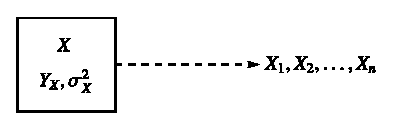
\includegraphics{figure/fig1.eps}}
\smallskip

and a function $w=h(x_{1},x_{2},\ldots,x_{n})$ of $n$ variables. Then (as we know) the combined random variable
$$
W=h(X_{1},X_{2},\ldots,X_{n})
$$
is called a {\it statistic.}
\end{frame}

\begin{frame}
If the population random variable $X$ is discrete then $X_{1},X_{2},\ldots,X_{n}$ will all be discrete and since $W$ is a combination of discrete random variables it too will be discrete.

\myheading{The \$64,000 question}

How is $W$ distributed ?

More precisely, what is the $pmf$ $P_{W}(x)$ of $W$.

The distribution $P_{W}(x)$ of $W$ is called a ``sampling distribution''.

Similarly if the population random variable $X$ is continuous we want to compute the $pdf$ $f_{W}(x)$ of $W$ (now it is continuous)
\end{frame}

\begin{frame}
We will jump to \$5.5.

The most common $h(x_{1},\ldots,x_{n})$ is a linear function
$$
h(x_{1},x_{2},\ldots,x_{n})=a_{1}x_{1}+\cdots+a_{n}x_{n}
$$
where
$$
W=a_{1}X_{1}+a_{2}X_{2}+\cdots+a_{n}X_{n}
$$

\setcounter{romanproposition}{11}
\begin{romanproposition}[page 219]\label{prop-L}
Suppose $W=a_{1}X_{1}+\cdots+a_{n}X_{n}$.

Then
\begin{itemize}
\item[(i)]
\begin{tabbing}
$E(W)$ \== $E(a_{1}X+\cdots+a_{n}X_{n})$\\[3pt]
       \>= $a_{1}E(X_{1})+\cdots+a_{n}E(X_{n})$
\end{tabbing}

\item[(ii)] If $X_{1}, X_{2},\ldots,X_{n}$ are independent then
$$
V(a_{1}X_{1}+\cdots+a_{n}X_{n})=a^{2}_{1}V(X_{1})+\cdots+a^{2}_{n}V(X_{n})
$$
(so $V(cX)=c^{2}V(X)$)
\end{itemize}
\end{romanproposition}
\end{frame}

\begin{frame}
\setcounter{romanproposition}{11}
\begin{romanproposition}[Cont.]
Now suppose $X_{1},X_{2},\ldots,X_{n}$ are a random sample from a population of mean $\mu$ and variance $\sigma^{2}$ so
\begin{align*}
& E(X_{i})=E(X)=\mu,\quad 1\leq i\leq n\\[3pt]
& V(X_{i})=V(X)=\sigma^{2},\quad 1\leq i\leq n
\end{align*}
and $X_{1}, X_{2},\ldots,X_{n}$ are independent.

We recall
\begin{align*}
T_{0} &= \text{the sample total } =X_{1}+\cdots+X_{n}\\[3pt]
\overline{X} &= \text{the sample mean } = \frac{X_{1}+\cdots+X_{n}}{n}
\end{align*}
\end{romanproposition}
\end{frame}

\begin{frame}
As an immediate consequence of the previous proposition we have

\begin{romanproposition}\label{prop-M}
Suppose $X_{1},X_{2},\ldots,X_{n}$ is a random sample from a population of mean $\mu_{X}$ and variance $\sigma^{2}_{X}$. Then
\begin{itemize}
\item[(i)] $E(T_{0})=n\mu_{X_{2}}$

\item[(ii)] $V(T_{0})=n\sigma^{2}_{X}$

\item[(iii)] $E(\overline{X})=\mu_{X}$

\item[(iv)] $V(\overline{X})=\dfrac{\sigma^{2}_{X}}{n}$
\end{itemize}
\end{romanproposition}
\end{frame}

\begin{frame}
\begin{nonumproof}[this is important]
\begin{itemize}
\item[(i)] 
\begin{tabbing}
$E(T_{0})$ \== $E(X_{1}+\cdots+X_{n})$\\[4pt]
                     \>by the Prop.\\[4pt]
                     \>= $E(X_{1})+\cdots+E(X_{n})$\\[4pt]
                     \>why\\[4pt]
                     \>= $\underbrace{\mu_{X}+\cdots+\mu_{X}}_{n\text{~copies}}$\\[4pt]
                     \>= $n\mu_{X}$
\end{tabbing}

\item[(ii)]
\begin{tabbing}
$V(T_{0})$ \== $V(X_{1}+\cdots+X_{n})$\\[4pt]
           \>\text{by the Prop}\\[4pt]
           \>= $V(X_{1})+\cdots+V(X_{n})$\\[4pt]
           \>= $\sigma^{2}_{X}+\cdots+\sigma^{2}_{X}$\\[4pt]
           \>= $n\sigma^{2}_{X}$
\end{tabbing}
\end{itemize}
\end{nonumproof}
\end{frame}

\begin{frame}
\begin{proof}[Proof (Cont.)]

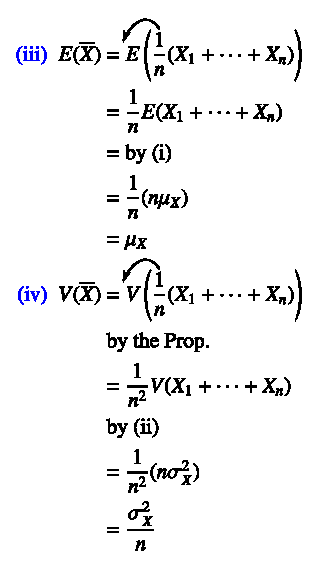
\includegraphics{figure/fig2.eps}
\end{proof}
\end{frame}

\begin{frame}
\begin{nonumremark}
It is important to understand the symbols -- $\mu_{X}$ and $\sigma^{2}_{X}$ are the mean and variance of the {\it underlying population.} 

In fact they are called the {\it population mean} and the {\it population variance}. Given a statistic $W=h(X_{1},\ldots,X_{n})$ we would like to compute $E(W)=\mu_{W}$ and $V(W)=\sigma^{2}_{W}$ in terms of the population mean $\mu_{X}$ and 
\end{nonumremark}
\end{frame}

\begin{frame}
\begin{nonumremark}[Cont.]
population variance $\sigma^{2}_{X}$.

So we solved this problem for $W=\overline{X}$ namely
$$
\mu_{\overline{X}}=\mu_{X}
$$
and
$$
\sigma^{2}_{\overline{X}}=\frac{1}{n}\sigma^{2}_{X}
$$
Never confuse population quantities with sample quantities.
\end{nonumremark}
\end{frame}

\begin{frame}
\begin{nonumcorollary}
\begin{tabbing}
$\sigma_{\overline{X}}$ \== the standard deviation of $\overline{X}$\\[4pt]
                     \>= $\dfrac{\sigma_{X}}{\sqrt{n}} =\dfrac{\text{population standard deviation}}{\sqrt{n}}$
\end{tabbing}
\end{nonumcorollary}

\begin{proof}
\begin{align*}
\sigma_{\overline{X}} &= \sqrt{V(\overline{X})}\\[3pt]
&= \sqrt{\dfrac{\sigma^{2}_{X}}{n}}\\[3pt]
&= \dfrac{\sqrt{\sigma^{2}_{X}}}{\sqrt{n}}=\dfrac{\sigma_{X}}{\sqrt{n}}
\end{align*}
\end{proof}
\end{frame}


\begin{frame}
\myheading{Sampling from a Normal Distribution}

\begin{nonumtheoremLCN}[Linear combination of normal is normal]\label{thm-LCN}
Suppose $X_{1},X_{2},\ldots,X_{n}$ are independent and 
$$
X_{1}\sim N(\mu,\sigma^{2}_{1}),\ldots,X_{n}\sim N(\mu_{n},\sigma^{2}_{n}).
$$
Let $W=a_{1}X_{1}+\cdots+a_{n}X_{n}$. Then 
$$
W\sim N(a_{1}\mu_{1}+\cdots+a_{n}\mu_{n}, a^{2}_{1}\sigma^{2}_{1}+\cdots+a^{2}_{n}\sigma^{2}_{n})
$$
\end{nonumtheoremLCN}

\begin{nonumproof}
At this stage we can't prove $W$ is normal (we could if we have moment
\end{nonumproof}
\end{frame}

\begin{frame}
\begin{proof}[Proof (Cont.)]
generating functions available).

But we can compute the mean and variance of $W$ using Proposition \ref{prop-L}.
\begin{align*}
E(W) &= E(a_{1}X_{1}+\cdots+a_{n}X_{n})\\[3pt]
     &= a_{1}E(X_{1})+\cdots+a_{n}E(X_{n})\\[3pt]
     &= a_{1}\mu_{1}+\cdots+a_{n}\mu_{n}
\end{align*}
and
\begin{align*}
V(W) &= V(a_{1}X_{1}+\cdots+a_{n}X_{n})\\[3pt]
     &= a^{2}_{1}V(X_{1})+\cdots+a^{2}_{n}V(X_{n})\\[3pt]
     &= a^{2}_{1}\sigma^{2}_{1}+\cdots+a^{2}_{n}\sigma^{2}_{n}
\end{align*}
\end{proof}
\end{frame}

\begin{frame}
Now We can state the theorem we need.

\setcounter{romantheorem}{13}
\begin{romantheorem}\label{thm-N}
Suppose $X_{1},X_{2},\ldots,X_{n}$ is a random sample from $N(\mu,\sigma^{2})$

\smallskip
\centerline{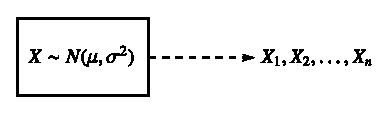
\includegraphics{figure/fig3.eps}}
\smallskip

Then
$$
T_{0}\sim N(n\mu, n\sigma^{2})
$$
and
$$
\overline{X}\sim N\left(\mu,\dfrac{\sigma^{2}}{n}\right)
$$
\end{romantheorem}

\begin{nonumproof}
The hard part is that $T_{0}$ and $\overline{X}$ are normal (this is Theorem LCN)
\end{nonumproof}
\end{frame}


\begin{frame}
\begin{proof}[Proof (Cont.)]
You show the mean of $\overline{X}$ is $\mu$ using either Proposition \ref{prop-M} or Theorem \ref{thm-LCN} and the same for showing the variance of $\overline{X}$ is $\dfrac{\sigma^{2}}{n}$.
\end{proof}

\begin{nonumremark}
It is very important for statistics that the sample variance
$$
S^{2}=\dfrac{1}{n-1}\sum\limits^{n}_{i=1}(X_{i}-\overline{X})^{2}
$$
satisfies
$$
S^{2}\sim \chi^{2}(n-1).
$$
This is one reason that the chi-squared distribution is so important.
\end{nonumremark}
\end{frame}

\begin{frame}
\myheading{3. The Central Limit Theorem (\S5.4)}

In Theorem \ref{thm-N} we saw that if we sampled $n$ times from a normal distribution with mean $\mu$ and variance $\sigma^{2}$ then
\begin{itemize}
\item[(i)] $T_{0}\sim N(n\mu, n\sigma^{2})$

\item[(ii)] $\overline{X}\sim N\left(\mu,\frac{\sigma^{2}}{n}\right)$
\end{itemize}

\myheading{So both $T_{0}$ and $\overline{X}$ are still normal}

The Central Limit Theorem says that if we sample $n$ times {\it with $n$ large enough} from {\it any distribution} with mean $\mu$ and variance $\sigma^{2}$ then $T_{0}$ has approximately $N(n\mu,n\sigma^{2})$ distribution and $\overline{X}$ has approximately $N(\mu,\sigma^{2})$ distribution.
\end{frame}

\begin{frame}
We now state the CLT.

\myheading{The Central Limit Theorem}

\smallskip
\centerline{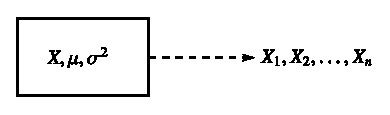
\includegraphics{figure/fig4.eps}}
\smallskip

$\overline{X}\approx N(\mu,\sigma^{2})$ provided $n>30$.

\begin{nonumremark}
This result would not be satisfactory to professional mathematicians because {\it there is no estimate of the error involved in the approximation.}  
\end{nonumremark}
\end{frame}


\begin{frame}
However an error estimate is known - you have to take a more advanced course.

The $n>30$ is a ``rule of thumb''. In this case the error will be neglible up to a large number of decimal places (but I don't know how many).

So the Central Limit Theorem says that for the purposes of sampling if $n>30$ then the sample mean {\it behaves as if the sample were drawn from a NORMAL population with the same mean and variation} of the actual population.
\end{frame}

\begin{frame}
\myheading{Example \thnum{5.27}\label{exam-5.27}}

A certain consumer organization reports the number of major defects for each new automobile that it tests. Suppose that the number of such defects for a certain model is a random variable with mean 3.2 and standard deviation 2.4. Among 100 randomly selected cars of this model what is the probability that the {\it average} number of defects exceeds 4.
\end{frame}

\begin{frame}
\begin{nonumsolution}
Let $X_{i}=\sharp$ of defects for the $i$-th car

\smallskip
\centerline{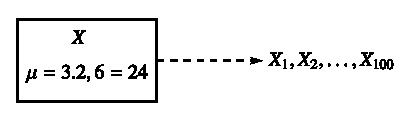
\includegraphics{figure/fig5.eps}}
\smallskip

$n=100>30$ so we can use the CLT
$$
\overline{X}=\dfrac{X_{1}+X_{2}+\cdots+X_{100}}{100}
$$
So
$$
\overline{X}=\text{average number of defects}
$$
So we want
$$
P(\overline{X}>4)
$$
\end{nonumsolution}
\end{frame}

\begin{frame}
\begin{nonumsolution}[Cont.]
Now 
\begin{align*}
E(\overline{X}) &= \mu=3.2\\[3pt]
V(\overline{X}) &= \dfrac{\sigma^{2}}{n}=\dfrac{(2.4)^{2}}{100}
\end{align*}
Let

\centerline{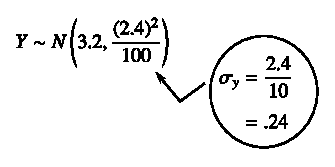
\includegraphics{figure/fig6.eps}}
\smallskip

By the CLT $\overline{X}\approx Y$ so

\smallskip
\centerline{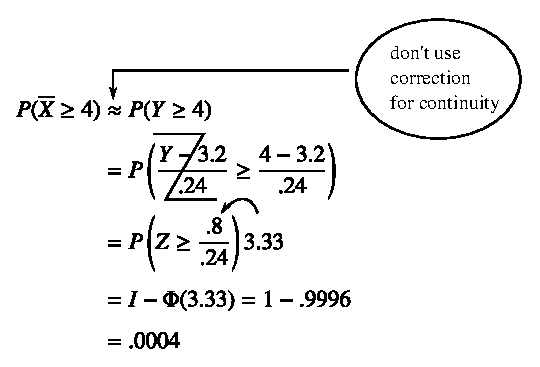
\includegraphics{figure/fig7.eps}}
\end{nonumsolution}
\end{frame}

\begin{frame}
\myheading{How the Central Limit Theorem Gets Used More Often}

The CLT is much more useful than one would expect. That is because many well-known distributions can be realized as sample totals of a sample drawn from another distribution. I will state this as

\myheading{General Principle}

Suppose a random variable $W$ can be realized as a sample total $W=T_{0}=X_{1}+\cdots+ X_{n}$ from some $X$ and $n>30$.

{\it Then $W$ is approximately normal.}
\end{frame}

\begin{frame}
\begin{nonumexamples}[This isn't ?????]
\begin{enumerate}
\item $W\sim \Bin (n,p)$ with $n$ large.

\item $W\sim \text{Gamma}(\alpha,\beta)$ with $\alpha$ large.

\item $W\sim \text{Poisson} (\lambda)$ with $\lambda$ large.
\end{enumerate}

We will do the example of $W\sim \Bin (n,p)$ and recover (more or less) the normal approximation to the binomial so
$$
\text{CLT} \Rightarrow \text{normal approx to binomial.}
$$
\end{nonumexamples}
\end{frame}

\begin{frame}
The point is

\begin{nonumtheorem}[sum of binomials is binomial]
Suppose $X$ and $Y$ are independent, $X\sim \Bin (m,p)$ and $Y\sim \Bin(n,p)$. Then 
$$
W=X+Y\sim \Bin (m+n,p)
$$
\end{nonumtheorem}

\begin{nonumproof}
For simplicity we will assume $p=\dfrac{1}{2}$.

Suppose Fred tosses a fair coin $m$ times and Jack tosses a fair coin $n$ times.
\end{nonumproof}
\end{frame}

\begin{frame}
\begin{proof}[Proof (Cont.)]
Let
\begin{align*}
X &= \sharp \text{~ of head Fred observes}\\[3pt]
Y &= \sharp \text{~ of heads Jack observes}
\end{align*}
So
$$
X\sim \Bin \left(m,\frac{1}{2}\right)\text{~~ and~~ } Y\sim \Bin \left(n,\frac{1}{2}\right)
$$
What is $X+Y$ ?

Forget who was doing the tossing, $X+Y$ is just the total number of heads in $m+n$ tosses of a fair coin so
$$
X+Y\sim \Bin \left(m+n,\frac{1}{2}\right).
$$
\end{proof}
\end{frame}

\begin{frame}
Now suppose we have

\smallskip
\centerline{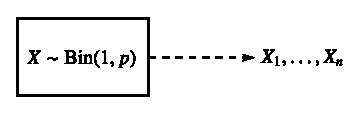
\includegraphics{figure/fig8.eps}}
\smallskip

Then $X_{i}\sim \Bin (1,p)$, $1\leq i\leq n$,
$$
T_{0}=X_{1}+X_{2}+\cdots+X_{n}\sim \Bin (n,p)
$$

Now if $n>30$ we know $T_{0}$ is approximately normal so if $W\sim \Bin (n,p)$ and $n>30$ the $W\approx$ normal
$$
E(W)=np\text{~~ and~~ } V(W)=npq\qquad\text{AND}
$$
\end{frame}

\begin{frame}
$$
W\sim N(np, npq)
$$
So we get the normal approximation to the binomial (with $n>30$ replacing $np\geq 10$ and $nq\geq 10$)

\begin{nonumremark}
If $p=\dfrac{1}{2}$ then the second conditions gives $n>20$.

- so better then CLT but if $p=\dfrac{1}{5}$ then the second conditions gives $n>50$.

- so worse than the CLT.
\end{nonumremark}
\end{frame}
\end{document}


